\section{FFS}
The artifact that was developed as a result of this thesis is the Fejk FileSystem (FFS). It used online services to store the data but behaved as a mountable filesystem for the users. The filesystem will be minimal and not support all functionalities that other filesystems do, such as links. The reasoning is that these behaviors are not required for a useable system, and when comparing the system to distributed filesystems such as Google Drive, many of these other filesystems also often do not support links.

\subsection{Design overview}
FFS uses images to store the data of files, directories and the inode table of the filesystem. These images will are uploaded to online web services, such as Flickr, as image posts. As mentioned in Section~\ref{sec:twitter}, there can be limitations to these posts for certain online web services. To support file sizes bigger than these limitations, bigger files will be split into multiple posts, requiring FFS to keep track of a list of posts. Figure~\ref{fig:ffs_inode_diag} presents the basic outline of FFS and a example content of the filesystem. FFS is based on the idea of inode filesystems and uses a inode table to store information about the files and directories in the filesystem. However, instead of an inode pointing to specific blocks in a disk, the inode table of FFS will instead keep track of the id numbers of the posts on the online services where the file or directory is located. The inode table entry for each file or directory will also contain metadata about the entry, such as its size and a boolean indicating if the entry is a directory or not.

\begin{figure}[!ht]
	\begin{center}
	  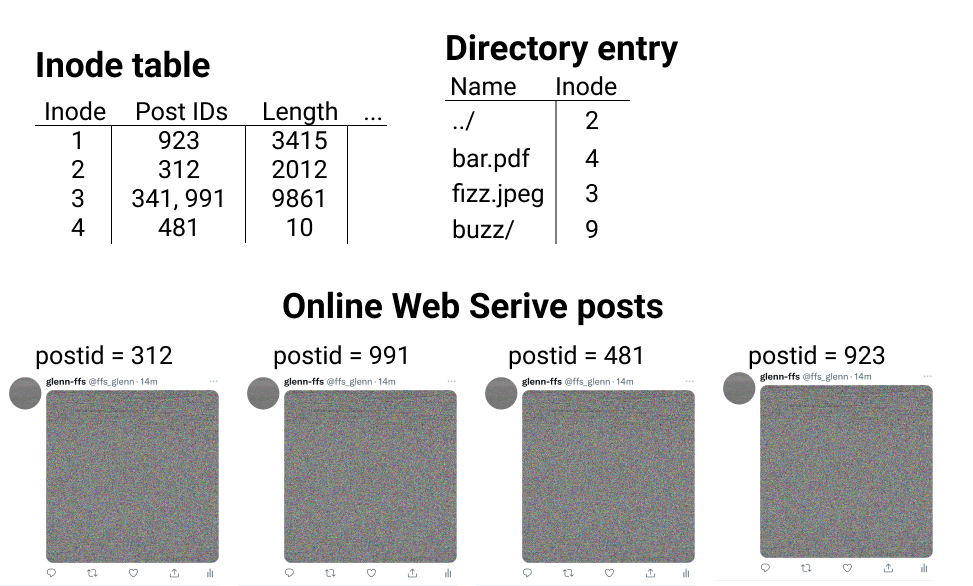
\includegraphics[width=0.8\textwidth]{figures/ffs_inode_diagram.png}
	\end{center}
	\caption{Basic structure of FFS inode-based structure}
	\label{fig:ffs_inode_diag}
\end{figure}

The directories and inode table are represented as classes in C++. Appendix~\ref{lst:dir_itable_classes} visualizes the main attributes of the \texttt{Directory}, \texttt{InodeTable}, and \texttt{InodeEntry} classes. There can be multiple \texttt{Directory} and \texttt{InodeEntry} objects in the computers' memory and in the filesystem, but there will only exist one \texttt{InodeTable} instance which is relevant. The \texttt{Directory} class is a data structure that stores mappings between filenames and the files' and directories' inode for all files and directories stored in that directory. The \texttt{InodeTable} stores a mapping between an inode and the files' \texttt{InodeEntry}. The \texttt{InodeEntry} is a data structure that keeps track of a file or directory's information, such as where the data is stored and its metadata, such as size and creation timestamp. To read the content of a known file in a directory therefore has three steps:
\begin{itemize}
	\item The \texttt{Directory} object of the directory provides the inode of the given filename.
	\item The inode is used to get the \texttt{InodeEntry} from the \texttt{InodeTable}.
	\item Using the inode entry, the location of the file can be located.
\end{itemize}
The location of a file or directory is an ordered list of unique IDs of the image posts on online web services. The data received by downloading these images, decoding them (as described in Subsection~\ref{subsec:file_enc_dec}), and concatenating them, can be read as a file or represented as a \texttt{Directory} object, depending on if the \texttt{InodeEntry} was marked as a file or a directory.

FFS does not support all filesystem operations that are implementable through FUSE, instead FFS implements a subset of them. The implemented functions are shown in Table~\ref{tbl:fs_impl_op}. The implemented operations are the most vital operations required for a working filesystem. Operations such as \texttt{chown} provides extended capabilities of the filesystem but these are not required for a proof-of-concept filesystem\textbf{REF FUSE CHEAT SHEET BY PROF.}. The functionality of the filesystem operations implemented by FFS and their implementation details are described in Subsection~\ref{subsec:file_op} .

\begin{table}[!ht]
	\begin{center}
		\caption{Filesystem operations implementable by FUSE that, and wether or not FFS implements them}
		\begin{tabular}{| c | c |}
			
			\hline
			\textbf{Filesystem operation} 	& \textbf{Implemented}\\
			\hline
			\hline
			\texttt{getattr} & Yes\\
			\texttt{fgetattr} & Yes\\
			\texttt{read} & Yes\\
			\texttt{readdir} & Yes\\
			\texttt{write} & Yes\\
			\texttt{create} & Yes\\
			\texttt{mkdir} & Yes\\
			\texttt{unlink} & Yes\\
			\texttt{rmdir} & Yes\\
			\texttt{rename} & Yes\\
			\texttt{truncate} & Yes\\
			\texttt{ftruncate} & Yes\\
			\texttt{statfs} & Yes\\
			\texttt{access} & Yes\\
			\texttt{flush} & Yes\\
			\texttt{utimens} & Yes\\
			\texttt{readlink} & No\\
			\texttt{opendir} & No\\
			\texttt{symlink} & No\\
			\texttt{link} & No\\
			\texttt{chmod} & No\\
			\texttt{chown} & No\\
			\texttt{open} & No\\
			\texttt{release} & No\\
			\texttt{released} & No\\
			\texttt{fsync} & No\\
			\texttt{fsyncdir} & No\\
			\texttt{lock} & No\\
			\texttt{bmap} & No\\
			\texttt{setxattr} & No\\
			\texttt{getxattr} & No\\
			\texttt{listxatt} & No\\
			\texttt{ioctl} & No\\
			\texttt{poll} & No\\
			\hline

		\end{tabular}
		\label{tbl:fs_impl_op}
	\end{center}
\end{table}

\subsection{Encoding and decoding objects}
\label{subsec:file_enc_dec}
Objects that FFS store, and therefore also encode and decode, are: files, directories and the inode table. All of these objects are stored on online web services using images. The inode table and the directories are represented as C++ objects in memory, but are serialized into a binary representation during runtime before encoded into images. The files saved to FFS are also read in to memory in a binary format before being encoded and uploaded to the online web services.

All FFS images are encoded in the same way, using a defined header in the beginning to inform the decoder of, among other things, the size of the encoded data. The decoder expects the header and will return an error if it is not correct. Further, the \texttt{Directory}, \texttt{InodeTable}, and \texttt{InodeEntry} classes are serialized into a binary format before they are uploaded to online web services. The binary data can be deserialized into the same object at a later time. A detailed description of these binary formats is described in Appendix~\ref{app:binary_rep}.


\subsection{Implemented filesystem operation}
\label{subsec:file_op}
% As a deniable filesystem, you should not be able to gain any information about the filesystem without the correct credentials. Using incorrect credentials, the filesystem will just show an empty filesystem meaning that the adversary will not know wether the credentials provided were correct and that the filesystem is empty, or if the credentials were incorrect. Only when the correct credentials are provided will FFS show the filesystem contents of the user.

